\documentclass{article}
\usepackage{maa-monthly}

%% IF YOU HAVE FONTS INSTALLED
%\usepackage{mtpro2}
%\usepackage{mathtime}

\theoremstyle{theorem}
\newtheorem{theorem}{Theorem}
 
\theoremstyle{definition}
\newtheorem*{definition}{Definition}
\newtheorem*{remark}{Remark}

\begin{document}

\title{An Alternative Geometric Interpretation of the Riemann-Stieltjes Integral}
\markright{Abbreviated Article Title}
\author{Trienko Lups Grobler}

\maketitle

\begin{abstract}
It is desirable to have geometric interpretations of difficult mathematical concepts. In this paper we present an intuitive geometric interpretation of the Riemann-Stieltjes integral. It can be 
summarized as follows: the Riemann-Stieltjes integral can be interpreted as an infinite sum of infinitesimally small non-rectangular 
integration strips. This interpretation is surprisingly similar to the geometric interpretation of the ordinary Riemann integral. 
It is therefore likely that students, encountering the Riemann-Stieltjes integral for the first time, would find this new alternative geometric framework a useful visualization tool.
\end{abstract}

\noindent
Providing a geometrical interpretation for a mathematical concept can greatly improve one's understanding of it. The Riemann-Stieltjes 
integral is no exception. G.~Bullock proposed a projection-based geometric framework with which one can interpret the Riemann-Stieltjes 
integral \cite{bullock1988}. Furthermore, I.~Podlubny proposed to interpret the Riemann-Stieltjes integral as the real distance covered by a moving object, whose speed was 
correctly recorded but at incorrect times \cite{podlubny2002}. In this paper we present an alternative, more initiative, geometric interpretation of the Riemann-Stieltjes integral.\\

\noindent
Ackermann et al. utilized the idea of using non-rectangular integration strips to perform integration
and in doing so developed the Cavalieri integral \cite{ackermann2012}. The area of a non-rectangular integration strip is computed via 
Cavalieri's principle \cite{andersen1985,eves1991, malik1984, wildberger2002, young1985}. They also showed that a Cavalieri integral can easily be converted to a Riemann-Stieltjes integral. 
However, the reverse operation was not described in \cite{ackermann2012}. In this paper we address this shortcoming. This 
reverse operation actually allows us to contrive a novel geometric interpretation of the Riemann-Stieltjes integral.
This geometric interpretation is: the Riemann-Stieltjes integral can be interpreted as an infinite sum of infinitesimally small
non-rectangular integration strips. Interestingly enough, this interpretation is very similar 
to the geometric interpretation of the Riemann integral. The priciple difference between these interprations is the shape of the ingration strips; non-rectangular in the case of the Riemann-Stieltjies integral and rectangular in the case of the Rieman integral.  
This rectangular geometric interpretation has been quite useful when 
teaching the ordinary Riemann integral to undergraduate students \cite{jones2015,sealey2014}. Consquently, it seems likely that undergraduate students would find the non-rectangular geometric interpretation
of the Riemann-Stieltjes integral just as useful. It is also interesting to mention that there are a few papers in the literature that propose teaching simpler integral definitions (which are easier to grasp) before introducing students to the Riemann integral \cite{czarnocha2001,prabhu2008,ruffa2002,zaskis2014}. It therefore also seems plausible that
students will find it useful to first understand the simpler Cavalieri integral before they are exposed to the more abstract Riemann-Stieltjes integral.\\

\noindent
We first present the formal definitions of the Riemann-Stieltjes and Cavalieri integrals \cite{bartle1976,ackermann2012}.
We then present the geometric interpretation proposed by G.~Bullock \cite{bullock1988}, which is followed up by the new alternative interpretation. We end 
the paper with some examples which aim to help the reader better understand and visualize the new alternative interpretation.

\section{Riemann-Stieltjes integral}
Let $f$ and $g$ denote real-valued functions defined on a closed interval $[a',b']$ of the real line. We shall suppose that 
both $f$ and $g$ are bounded on $[a',b']$. 

\begin{definition}
Define a partition $\mathcal{P}$ of $[a',b']$ to be a set of points $x_0, x_1,\cdots,x_n$, 
where $a' = x_0 \leq x_1 \leq \cdots \leq x_n = b'$. For each partition 
$\mathcal{P}$ of $[a',b']$ write $\Delta g_k = g(x_k)-g(x_{k-1})$. Let 
$M_k = \sup\{f(x),x_{k-1}\leq x \leq x_{k}\}$, $m_k = \inf\{f(x),x_{k-1}\leq x \leq x_{k}\}$, and set 
\begin{equation}
\label{ref:S_up}
\mathcal{S}_U(\mathcal{P},f,g) = \sum_{k=1}^n M_k \Delta g_k, 
\end{equation}
and
\begin{equation}
\label{ref:S_low}
\mathcal{S}_L(\mathcal{P},f,g) = \sum_{k=1}^n m_k \Delta g_k. 
\end{equation}
The sums in Eq.~\eqref{ref:S_up} and Eq.~\eqref{ref:S_low} are respectively called the the upper and lower Riemann-Stieltjes sums.
If there is a unique number $I$ that satisfies the inequality $\mathcal{S}_L(\mathcal{P},f,g)\leq I \leq \mathcal{S}_U(\mathcal{P},f,g)$ for all 
partitions $P$ of $[a',b']$, then $f$ is Riemann integrable with respect to $g$ on $[a',b']$. Moreover, $I$ is called the Riemann-Stieltjes integral of $f$ from $a'$ to $b'$ and is denoted by
\begin{equation}
\int_{a'}^{b'} f(x) dg(x). 
\end{equation}
\end{definition}

\begin{theorem}
If the derivative $g'$ exists and is continuous on $[a',b']$ and if $f$ is integrable with respect to $g$ on $[a',b']$, then the following 
Riemann and Riemann-Stieltjes integrals are equivalent
\begin{equation}
\int_{a'}^{b'} f(x) dg(x) = \int_{a'}^{b'} f(x)g'(x)dx.
\end{equation}
\end{theorem}

%\begin{theorem}
%Assume $g(x)$ increases monotonically and $g'(x)$ is Riemann intergable on $[a,b]$. Let $f$ be a bounded, real, Riemann integrable 
%function on $[a,b]$. Then
%\begin{equation}
%\int_a^b f dg(x) = \int_a^b f(x) g'(x) dx. 
%\end{equation}
%\end{theorem}

%\begin{theorem}
%If $a'<s<b'$, $f$ is continuous at $s$, and 
%\begin{equation}
%g(x) = 
%\begin{cases}
%0 & \textrm{if}~x\leq s\\
%1 & \textrm{if}~x > s
%\end{cases}
%\end{equation}
%then $\int_a^b f dg(x) = f(s)$.
%\end{theorem}

% #########################################################################################################
% Bartle definition of Riemann-Stieltjes integral
% #########################################################################################################

% \subsection{Bartle s. 29 p. 212}
% Let $f$ and $g$ denote real-valued functions defined on a closed interval $J=[a,b]$ of the real line. We shall suppose that 
% both $f$ and $g$ are bounded on $J$. A partition of $J$ is a finite collection  of non-overlapping intervals whose union is $J$. 
% Usually, we describe a partition $P$ by specifying a finite set of real numbers $(x_0,x_1,\cdots,x_n)$ such that 
% \begin{equation}
% a = x_0 \leq x_1 \leq \cdots \leq x_n = b
% \end{equation}
% and such that the subintervals occuring in the partition $P$ are the intervals $[x_{k-1},x_k]$, $k = 1,2,\cdots,n$. Hence we write 
% $P = (x_0,x_1,\cdots,x_n)$. If $P$ and $Q$ are partitions of $J$, we say $Q$ is a refinement of $P$ or that $Q$ is finer than $P$ in case every subinterval in $Q$ is contained in some subinterval in $P$.
% 
% \begin{definition}
% If $P$ is a partition of $J$, then a Riemann-Stieltjes sum of $f$ with respect to $g$ and corresponding to $P$ is a real number 
% $S(P,f,g)$ of the form 
% \begin{equation}
% S(P,f,g) = \sum_{k=1}^n f(\xi_{k})\{g(x_k)-g(x_{k-1})\}. 
% \end{equation}
% Here we have selected numbers $\xi_{k}$ satisfying 
% \begin{equation}
% x_{k-1} \leq \xi_{k} \leq x_{k}~\textrm{for}~k=1,2,\cdots,n.  
% \end{equation}
% \end{definition}
% 
% \begin{definition}
% We say that $f$ is integrable with respect to $g$ on $J$ if there exists a real number $I$ such that for every number $\epsilon>0$ there 
% is a partition $P_{\epsilon}$ of $J$ such that if $P$ is a refinement of $P_{\epsilon}$ and $S(P,f,g)$ is any Riemann-Stieltjes sum corresponding 
% to $P$, then 
% \begin{equation}
% |S(P,f,g)-I|<\epsilon. 
% \end{equation}
% In this case the number is uniquely determined and is denoted by
% \begin{equation}
% I = \int_a^b f(x) dg(x). 
% \end{equation}
% \end{definition}
% 
% \begin{theorem}
% If the derivative $g'$ exists and is continious on $J$ and if $f$ is integrable with respect to $g$, then the product $fg'$ is Riemann
% integrable and 
% \begin{equation}
% \int_a^b f(x) dg(x) = \int_a^b f(x)g'(x)dx.
% \end{equation}
% \end{theorem}

\section{Cavalieri integral}
Let $a(y)$ be a translational function with respect to a function $f(x)$ on the interval $[a,b]$. Moreover, $b(y) := a(y) + (b-a)$. Furthermore, the functions $a(y)$ and $b(y)$ intersect $f(x)$ at $a'$ and $b'$ respectively.
These assertions are assumed to be true throughout the paper and will not be repeated again.

\begin{definition}[Translational Function]
A continuous real-valued function $a(y)$ is called a translational function with respect to a continuous real-valued function $f(x)$ on the interval $[a,b]$ if 
$\{x\in\mathbb{R}|a\circ f(x) + z = x\}$ is a singleton, for every $z\in[0,b-a]$ and $a(0) = a$.
\end{definition}

\begin{definition}[Transformation Function]
The mapping $h : [a, b] \rightarrow [a',b']$, which maps $x_i^1 \in [a, b]$ to $x_i^2 \in [a',b']$, is defined as
$h(x_i^1) :=$ $\{x_i^2 \in [a' ,b'] | a\circ f(x_i^2) + [x_i^1 - a] = x_i^2$ , $a = a(0)\}$
\end{definition}

\noindent
It can easily be shown that $h(x)$ is a strictly monotone continuous function. It is therefore also bijective. 

\begin{definition}[Inverse Transformation Function]
The mapping $g:[a', b'] \rightarrow [a, b]$, which maps $x_i^2 \in [a' , b']$ to $x_i^1\in [a, b]$,
is defined as $g(x_i^2) := x_i^2 - a \circ f (x_i^2) + a$.
\end{definition}

\noindent
Note, that $g = h^{-1}$ per definition. Moreover $g$ is guaranteed to exist, since $h$ is bijective. 

\begin{definition}
Define a partition $\mathcal{P}_1$ of $[a,b]$ to be a set of points $x_0, x_1,\cdots,x_n$, 
where $a = x_0^1 \leq x_1^1 \leq \cdots \leq x_n^1 = b$. For each partition 
$\mathcal{P}_1$ of $[a,b]$ write $\Delta x_k = x_k-x_{k-1}$. 
%Since both boundaries of any integration strip are necessarily
%translations of the translational function $a(y)$, we can apply the transformation
%function $h$ to the partition $\mathcal{P}_1$. 
If the transformation function $h$ is strictly increasing,
the application of $h$ to the partition $\mathcal{P}_1$ induces a new partition $\mathcal{P}_2 = \{x_0^2, x_1^2,\cdots, x_n^2\}$.
Otherwise, if $h$ is strictly decreasing, the application of $h$ induces a reversed partition $\mathcal{P}_2 = \{x_n^2, \cdots, x_1^2,x_0^2\}$. It
can be assumed that $h$ is strictly increasing, without any loss of generality.  Let 
$M_k = \sup \{f (x), h(x_{i-1}^1) = x_{i-1}^2 \leq x \leq x_i^2 = h(x_i^1)\}$, $m_k = \inf \{f (x), h(x_{i-1}^1) = x_{i-1}^2 \leq x \leq x_i^2 = h(x_i^1)\}$, and set 
\begin{equation}
\label{eq:c_up}
\mathcal{C}_U(\mathcal{P}_1,f,h) = \sum_{k=1}^n M_k \Delta x_k, 
\end{equation}
and
\begin{equation}
\label{eq:c_low}
\mathcal{C}_L(\mathcal{P}_1,f,h) = \sum_{k=1}^n m_k \Delta x_k. 
\end{equation}
The sums in Eq.~\eqref{eq:c_up} and Eq.~\eqref{eq:c_low} are respectively called the the upper and lower Cavalieri sums.
If there is a unique number $I$ that satisfies the inequality $\mathcal{C}_L(\mathcal{P}_1,f,h)\leq I \leq \mathcal{C}_U(\mathcal{P}_1,f,h)$ for all 
partitions $\mathcal{P}_1$ of $[a,b]$, then $I$ is called the Cavalieri integral of $f$ from $a(y)$ to $b(y)$ and is denoted by
\begin{equation}
\int_{a(y)}^{b(y)} f(x) dx.
\end{equation}
\end{definition}

\begin{theorem}
The following Cavalieri, Riemann and Riemann-Stieltjes integrals are equivalent
\begin{equation}
\int_{a(y)}^{b(y)} f(x) dx = \int_a^b f\circ h(x) dx = \int_{a'}^{b'} f(x)dg(x). 
\end{equation}
\end{theorem}

\begin{remark}
Note that the definition of the Cavalieri integral as presented above imposes much stricter requirements on $f$ and $g$ than the 
definition of the Riemann-Stieltjes integral does. To ensure consistency, we will assume, from here onwards and unless stated otherwise, that the stricter requirements imposed 
by the Cavalieri definition are now also binding on the Riemann-Stieltjes integral. Recall that the main aim of the paper is to 
help students develop a geometric intuition for the Riemann-Stieltjes integral that will be valid for most of the 
Riemann-Stieltjes integral problems that students will encounter during their undergraduate studies.
While this does not imply that this interpretation cannot provide insight into a broad range of problems, it does mean that the interpretation may not remain valid for each and every Riemann-Stieltjes integral
and not to present a complete geometric framework. This is not to say that the geometric interpretation presented here cannot be used to provide 
insight to a broad range of problems. In the example section we show that Cavalieri sums can provide meaningful insights even 
when we relax some of the strict restrictions imposed by the above definitions.
\end{remark}

\section{Cavalieri Integral: Example}

Consider the region $R$ bounded by the $x$-axis and the lines $f(x)=x$, $a(y)=1-y$ and $b(y)=4-y$. This region is shown in Fig.~\ref{fig:ex1}.\\
\begin{figure}[htb]
\centering
\includegraphics[width=0.36\textwidth]{fig12}
\caption{Region bounded by the $x$-axis and the lines $f(x)=x$, $a(y)=1-y$, and $b(y)=4-y$.}
\label{fig:ex1}
\end{figure}

\noindent
Instead of trying to determine the area of $R$ using rectangular integration strips, it seems more natural 
to use integration strips whose sides are translations of $a(y)$. Cavalieri's principle tells us that the area of an 
arbitrary shaped integration strip is the product of its height and the length of its base. The area of $R$ 
can be approximated by summing together multiple non-rectangular integration strips that inscribe $R$. This concept is illustrated in Fig.~\eqref{fig:caval2}. 
More formally, consider a partition $(x_i^1)_{i=0}^{n}$, on the $x$-axis, such that $a = x_0^1 < x_1^1 < \cdots < x_n^1 = b$, and $\Delta x_i^1 = x_{i+1}^1 - x_i^1$.
%As Fig.~\ref{fig:caval2} illustrates, the partition points $x_i^1$ are chosen to coincide with the $x$-coordinates at which the sides of the 
%integration strips intersect the $x$-axis. Fig.~\ref{fig:caval2} also shows us that another partition $(x_i^2)_{i=0}^{n}$, on the $x$-axis, such that $a' = x_0^2 < x_1^2 < \cdots < x_n^2 = b'$
%is automatically created when we make use of non-rectangular integration strips. The partition points $x_i^2$ 
%coincide with the $x$-coordinates at which the sides of the 
%integration strips intersect $f(x)$. 
Let us now construct the following sum (i.e. a lower Cavalieri sum) with which we can approximate the area 
of $R$:
\begin{equation}
\label{eq:cav_sum}
\sum_{i=0}^{n-1} f(x_i^2)\Delta x_i^1.
\end{equation}
The partition points $(x_i^2)_{i=0}^{n}$ are depicted in Fig.~\ref{fig:caval2}.
The above sum can be interpreted as summing together the areas associated with $n$ non-rectangular integration strips.
The left panel of Fig.~\ref{fig:caval2} depicts the scenario in which we made use of three integration strips.  
The right panel of Fig.~\ref{fig:caval2} illustrates that the larger $n$ becomes the better Eq.~\eqref{eq:cav_sum} approximates the area of $R$. In the limit Eq.~\eqref{eq:cav_sum} approaches the Cavalieri integral:
\begin{equation}
\label{eq:caval1}
\int_{a(y)}^{b(y)}f(x)\, dx = \lim_{n\to \infty}\sum_{i=0}^{n-1} f(x_i^2)\Delta x_i^1.
\end{equation}

\begin{figure}[htb]
\centering
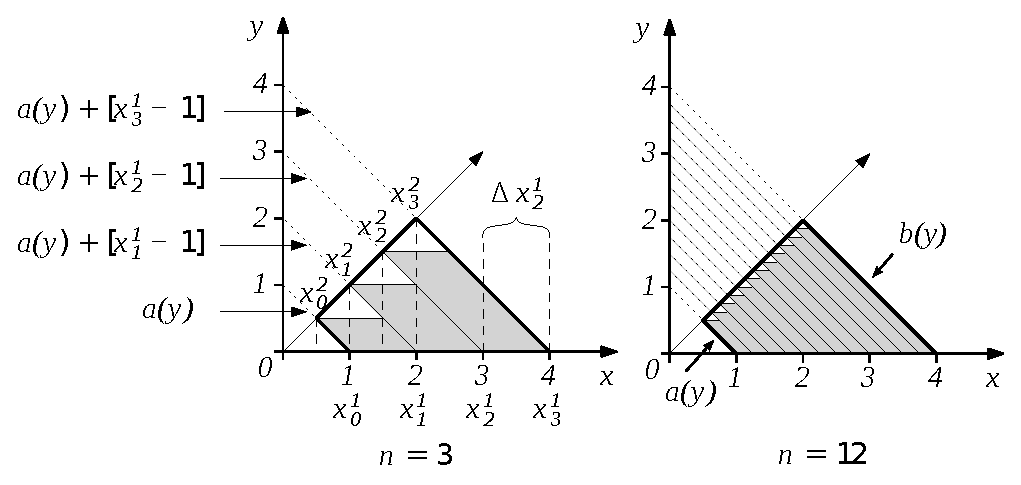
\includegraphics[width=0.92\textwidth]{fig13}
\caption{Partition points $x_i^2$ as used in the Cavalieri sum.}
\label{fig:caval2}
\end{figure}

\noindent
It is however hard to evaluate Eq.~\eqref{eq:caval1} in its present form. Fortuitously, we can transform the Cavalieri sum given in Eq.~\eqref{eq:caval1} into an ordinary Riemann sum
if we can determine an expression for $x_i^2$ in terms of the partition points $x_i^1$, for all $i=0,1,\ldots,n$. Consider the collection of functions $\{a(y) + [x_i^1-a] = x_i^2: i=0,1,\ldots,n\}$. To find the partition points $x_i^2$ in terms of $x_i^1$ we substitute the function $f(x_i^2)$ for $y$ to obtain:
\begin{align*}
a\circ f (x_i^2)+[x_i^1-1] &= x_i^2\\
x_i^2 &= \dfrac{x_i^1}{2},
\end{align*}
so that we have the general expression $x_i^2=h(x_i^1)$, with $h(x)=x/2$.\\

\noindent
The function $h$ allows us to rewrite the Cavalieri integral as an equivalent Riemann integral:
\begin{equation}
\label{eq:h_int}
\lim_{n\to \infty}\sum_{i=0}^{n-1} f(x_i^2)\Delta x_i^1 =  \lim_{n\to \infty}\sum_{i=0}^{n-1} f \circ h (x_i^1)\Delta x_i^1 = \int_a^b f \circ h (x)\, dx.
\end{equation}

\noindent
It is now possible to compute the Cavalieri integral by evaluating its equivalent Riemann integral:
\begin{equation}
\int_{a(y)}^{b(y)}f(x)\, dx = \int_a^b f \circ h (x)\, dx = \dfrac{1}{2}\int_1^4x\, dx = 3.75.  
\end{equation}

\noindent
Interestingly, the function $g=h^{-1}$ allows us to rewrite the Cavalieri integral as an equivalent Riemann-Stieltjes integral:
\begin{equation}
\label{eq:g_int}
\lim_{n\to \infty}\sum_{i=0}^{n-1} f(x_i^2)\Delta x_i^1 =  \lim_{n\to \infty} \sum_{i=0}^{n-1} f(x_i^2)[g(x_{i+1}^2)-g(x_{i}^2)] = \int_{a'}^{b'} f \, dg(x). 
\end{equation}

\noindent
We can therefore also compute the Cavalieri integral by evaluating its equivalent Riemann-Stieltjes integral:
\begin{equation}
\int_{a(y)}^{b(y)}f(x)\, dx = \int_{a'}^{b'} f \, dg(x) = \int_{\frac{1}{2}}^2x\, d2x = 3.75.  
\end{equation}

\noindent
We can quickly verify this to be correct by evaluating the area of $R$ with ordinary Riemann integration:
\begin{equation}
\int_0^2x\, dx+\int_2^44-x\, dx- \int_0^{\frac{1}{2}}x\, dx-\int_{\frac{1}{2}}^11-x\, dx = 3.75. 
\end{equation}

%Now consider the Riemann-Stieltjes integral: $\int_{a'}^{b'} f(x) dg(x)$. 
%In this figure $f(x) = x$, $g(x) = 2x$, $h(x) = \frac{1}{2}x$ and $a(y)=1-y$.

\section{Existing Geometric Interpretation}
G.~Bullock proposed one possible geometric interpretation of the Riemann-Stieltjes integral \cite{bullock1988}. 
The basic idea behind his approach is to represent $f(x)$ and $g(x)$ as three-dimensional sheets. 
The three dimensional coordinate system which G.~Bullock proposes to realize this representation is depicted in 
Fig.~\ref{fig:bullock}. The $f$-sheet is constructed by simply extending the curve $f$ which resides in the $fx$-plane 
along the $g$-direction. The $g$-sheet is constructed similarly. Note that, as $f$ is independent of $g$, the $f$-sheet remains 
constant along the $g$-direction. Similarly, the $g$-sheet remains constant along the $f$-direction. 
A new sheet, known simply as the ``fence'', can be created by chopping off any part of the $g$-sheet that protrudes above the 
$f$-sheet and below the $gx$-plane. This sheet can now be projected onto the $fg$-plane. The area of the region that is formed 
via this projection can be interpreted as the value which is obtained when the Riemann-Stieltjes integral is evaluated.\\ 

\noindent
Let us now try to make the above ideas more concrete by applying them to an example. Let $f(x)=x^2$ and 
$g(x)=x$. The sheets associated with these two functions are depicted in Fig.~\ref{fig:bullock}. 
The $f$-sheet is depicted in blue, while the $g$-sheet is red. The ``fence'' is depicted in green. The region
obtained by projecting the ``fence'' on to the $fg$-plane is depicted in black.\\

\noindent
\begin{remark}
It is interesting to note that G.~Bullock follows route similar to ours when developing his geometrical framework.
He starts of with quite strict requirements for $f$ ang $g$ and relaxes more and more of these requirements in his latter 
examples. 
\end{remark}

\begin{figure}[htb]
\centering
\includegraphics[width=1.0\textwidth]{3D_final-crop.pdf}
\caption{An example of using G.~Bullocks' geometric framework to interpret the Riemann-Stieltjes integral. In this example 
$f(x)$ is represented by the blue sheet and $g(x)$ is represented by the red sheet. Moreover, $f(x)=x^2$ and $g(x)=x$. The green sheet, simply known as the ``fence'', is formed 
by chopping off any part of the $g$-sheet which protrudes above the $f$-sheet and below the $gx$-plane. Projecting the ``fence''
onto the $fg$-plane produces the visible gray region in the $fg$-plane. The area of this gray region in the $fg$-plane is equal to the Riemann-Stieltjes integral:
$\int_{0}^{3} f(x) dg(x)$.}
\label{fig:bullock}
\end{figure}

\section{Alternative Geometric Interpretation}
\begin{figure}[htb]
\centering
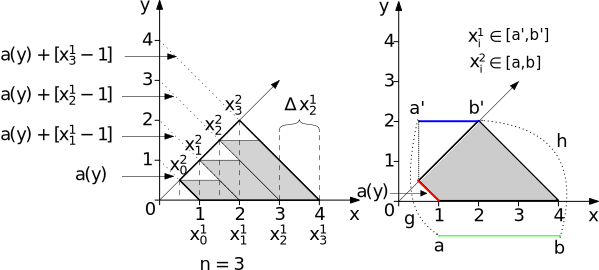
\includegraphics[width=1\textwidth]{fig13_change}
\caption{A non-rectangular sum-based geometric interpretation of the Riemann-Stieltjes integral. Moreover, the figure depicts the region $R$ (also see Fig.~\ref{fig:ex1}). The integrator $g$ maps points 
in $[a',b']$ (depicted in blue) to points in $[a,b]$ (depicted in green). The function $h$ performs the reverse operation. Moreover, $g$ maps the $x$-coordinates at which
translations of $a(y)$ (depicted in red) intersect with $f(x)$ to the $x$-intercepts of the translated functions. This observation enables us to interpret the Riemann-Stieltjes integral as an infinite sum of infinitesimally small non-rectangular integration 
strips.}
\label{fig:2d_geo}
\end{figure}
%\begin{equation}
%\label{eq:cal_def_2D}
%\int_{a(y)}^{b(y)}fdx =\lim_{n\to \infty}\sum_{i=0}^{n-1} f(x_i^2)\Delta x_i^1,
%\end{equation}
%and that
%\begin{equation}
%\label{eq:rs_def_g}
%\int_{a'}^{b'} f \, dg(x) = \lim_{n\to \infty} \sum_{i=0}^{n-1} f(x_i^2)[g(x_{i+1}^2)-g(x_{i}^2)].
%\end{equation}
%Fig.~\ref{fig:2d_geo} depicts a region whose area can be determined by considering non-rectangular integration strips.
%. Note that the shape of the integration strips are determined by $a(y)$. 
%In Fig.~\ref{fig:2d_geo}, the function $a(y)$ is depicted in red. If we translate $a(y)$ along the $x$-axis we actually create two partitions on the $x$-axis, 
%i.e. $(x_i^1)_{i=0}^{n}$ and $(x_i^2)_{i=0}^{n}$ with $x_i^1\in[a,b]$ and $x_i^2\in[a',b']$.  To map partition points in $[a',b']$ to partition points 
%in $[a,b]$ we use the function $g$. The reverse is achieved through $h$. The functions $g$ and $h$ depend soly on $a(y)$ and are also 
%computed with it.
Consider the definition of the Riemann-Stieltjes integral and 
Eq.~\eqref{eq:g_int}. For the sake of continiuty we repeat Eq.~\eqref{eq:g_int} below:
\begin{equation}
\label{eq:g_int2}
\int_{a'}^{b'} f(x) dg(x) =  \lim_{n \rightarrow \infty}\sum_{i=0}^{n-1} f(x_i^2)[g(x_{i+1}^2)-g(x_{i}^2)], 
\end{equation}
with $(x_i^2)_{i=0}^n$ being arbitrary partition points on the $x$-axis.
Eq.~\eqref{eq:g_int2} tells us that the function of the integrator $g$ is to map points in the interval $[a',b']$ to other 
locations on the $x$-axis. When, $g$ is monotone increasing it maps points in the interval $[a',b']$ to $[a,b]$,
with $a = g(a')$ and $b = g(b')$.\\

\noindent
To improve our understanding of $g$ lets investigate a specific example of the Riemann-Stieltjes integral in more depth: 
\begin{equation}
R = \int_{\frac{1}{2}}^1 x~d2x. 
\end{equation}
$R$ is depicted in Fig.~\ref{fig:2d_geo}. In this example $g$ maps $[\frac{1}{2},2]$ to $[1,4]$. The mapping between these two intervals is also 
depicted in Fig.~\ref{fig:2d_geo}. Moreover, the interval $[\frac{1}{2},2]$ is depicted in blue,
while the interval $[1,4]$ is depicted in green.\\ 

\noindent
Furthermore, consider $a(y) = 1-y$ (depicted in red in Fig.~\ref{fig:2d_geo}). Interestingly, the integrator $g$ maps the $x$-coordinates where translations of $a(y)$ and $f(x)$ intersect to the $x$-intercepts of the translations of $a(y)$.
The implications of this observation are the following: 
\begin{itemize}
 \item $g(x_{i+1}^2)-g(x_{i}^2)$ (i.e. $\Delta x_i^1$) represents the length of the base of a non-rectangular integration strip. Note, the base lengths in Fig.~\ref{fig:2d_geo} are all equal.
 \item $f(x_i^2)$ is the height of a non-rectangular integration strip.
 \item $f(x_i^2)[g(x_{i+1}^2)-g(x_{i}^2)]$ is the area of a non-rectangular integration strip (due to Cavalieri's principle).
 \item The Riemann-Stieltjes sum, i.e. $\sum_{i=0}^{n-1} f(x_i^2)[g(x_{i+1}^2)-g(x_{i}^2)]$, is equal to the area obtained by summing together the area of multiple 
 integration strips.
 \item In the limit the Riemann-Stieltjes sum approaches $R$. 
\end{itemize}
The Riemann-Stieltjes integral can therefore be interpreted as the area which is obtained by summing together the areas of an infinite number of infinitesimally small non-rectangular integration strips,
i.e. a Riemann-Stieltjes integral can be converted into an equivalent Cavalieri integral.\\

%Consider Fig.~\ref{fig:2d_geo}, whilst keeping in mind the definition of the Riemann-Stieltjes integral presented in 
%Eq.~\eqref{eq:g_int}. For the sake of continiuty we repeat this definition below:
%\begin{equation}
%\label{eq:g_int2}
%\int_{a'}^{b'} f(x) dg(x) =  \lim_{n \rightarrow \infty}\sum_{i=0}^{n-1} f(x_i^2)[g(x_{i+1}^2)-g(x_{i}^2)]. 
%\end{equation}
%Fig.~\ref{fig:2d_geo} depicts the same region we used to explain the Cavalieri integral a bit better (see Fig.~{}).\\

%\noindent
%In light of the above equation and Fig.~\ref{fig:2d_geo}, how then should we interpret the Riemann-Stieltjes integral of $f$ 
%with respect to $g$ over the interval $[a',b]$? Eq.~\eqref{eq:g_int2} tells us that the function of the integrator $g$ is to map points in the interval $[a',b']$ to other 
%locations on the $x$-axis. When, $g$ is monotone increasing it maps points in the interval $[a',b']$ to $[a,b]$,
%with $a = g(a')$ and $b = g(b')$. For the specific example presented in Fig.~\ref{fig:2d_geo}, we can actually go one step 
%further. The integrator $g$ maps the $x$-coordinates where translations of $a(y)$ and $f(x)$ intersect to the $x$-intercepts of the translated functions intersect the $x$-axis.
%The implications of this assertion is the following: 
%\begin{itemize}
% \item $g(x_{i+1}^2)-g(x_{i}^2)$ represents the length of the base of a non-rectangular integration strip.
% \item $f(x_i^2)$ is the height of a non-rectangular integration strip.
% \item $f(x_i^2)[g(x_{i+1}^2)-g(x_{i}^2)]$ is the area of a non-rectangular integration strip (due to Cavalieri's principle).
% \item The Riemann-Stieltjes sum, i.e. $\sum_{i=0}^{n-1} f(x_i^2)[g(x_{i+1}^2)-g(x_{i}^2)]$, is equal to the area obtained by summing together the area of multiple 
% integration strips.
% \item In the limit the Riemann-Stieltjes sum approaches the area of $R$. 
%\end{itemize}
%The Riemann-Stieltjes integral, can therefore, be interpreted as the area which is obtained, by summing together the areas of an infinite number of infinitesimally small non-rectangular integration strips,
%i.e. a Riemann-Stieltjes integral can be converted into an equivalent Cavalieri integral.\\

\noindent
The geometric interpretation provided above was possible due to the fact that the function $a(y)$
was known to us a priori. In general $a(y)$ will be unknown. Below we discuss how $a(y)$ can be computed.\\

%the Riemann-Stieltjes sumthe Riemann-Stieltjes 
%In the original Cavalieri paper only the forward direction is discussed: given $a(y)$ how do we obtain $g(x)$. Being able to 
%go in the other direction is crucial if we wish to provide a geometric interpretation of the Riemann-Stieltjes integral using an infinite sum.
%Below we address this short-coming.\\ 

\noindent
For all $C \in \mathbb{R}$ we have that
\begin{equation}
\label{eq:rs_C}
\int_{a'}^{b'} f(x)dg(x) = \int_{a'}^{b'} f(x)d[\widetilde{g}(x)+C], 
\end{equation}
with $g(x) := \widetilde{g}(x)+C$. 
Moreover, 
\begin{equation}
\label{eq:g_x_start}
g(x) =  x - a\circ f(x) + a.
\end{equation}
It would seem that we are unable to calculate $a(y)$, since we do not know the value 
of $a$ nor $C$ a priori. However, we do know that 
\begin{equation}
g(a') = \widetilde{g}(a') + C = a \implies C = a - \widetilde{g}(a'). 
\end{equation}
If we substitute $C$ with $a - \widetilde{g}(a')$ in Eq.~\eqref{eq:g_x_start} we eliminate both $C$ and $a$ from it. This 
substitution results in
\begin{equation}
\widetilde{g}(x) - \widetilde{g}(a') =  x - a\circ f(x).
\end{equation}
The above equation can be rewritten as
\begin{equation}
a\circ f(x) = x - \widetilde{g}(x) + \widetilde{g}(a').   
\end{equation}
If we now substitute $x$ with $f^{-1}(y)$ we obtain an expression for $a(y)$
\begin{equation}
a(y) = f^{-1}(y) - \widetilde{g}\circ f^{-1}(y) + \widetilde{g}(a').   
\end{equation}

\noindent
Once we have an expression for $a(y)$ we can trivially compute the following values and expressions:
\begin{itemize}
 \item Compute $a = a(0)$.
 \item Compute $C = a - \widetilde{g}(a')$.
 \item Compute $b = g(b')$ and $b(y) = a(y) + (b-a)$.
 \item Compute $h(x) = g^{-1}(x)$. 
\end{itemize}

\begin{remark}
Note that the above procedure places an even stricter limitation on $f$, it now also needs to be invertible. Moreover the 
above derivation also requires that $a(0)$ exists.
\end{remark}

%\noindent
%The above values and expressions enable us to convert Eq.~\ref{eq:rs_C} into a Cavalieri integral, i.e. 
%\begin{equation}
%\int_{a'}^{b'} f(x)dg(x) = \int_{a(y)}^{b(y)} f(x) dx. 
%\end{equation}
%\noindent
%The implication being, that the Riemann-Stieltjes integral can be interpreted as an infinite sum of infinitesimally small integration strips.
%The integration strips are however not rectangular as is the case for an ordinary Riemann integral, but have a shape which is determined by the function $a(y)$.

\section{Examples}
A couple of Riemann-Stieltjes integrals are given in Table~\ref{tab:table1}. The $a(y)$ functions associated 
with these Riemann-Stieltjes integrals are presented in the same table and were computed using the method 
described in the previous section. The Riemann-Stieltjes integrals were also evaluated using both $g$ and $h$ and the result
thereof is reported in Table~\ref{tab:table2}. The non-rectangular sum-based geometric interpretations of the integrals in Table~\ref{tab:table1} are depicted in Figs.~\ref{fig:ex1_sec}--\ref{fig:ex4_sec}.\\

\noindent
In Fig.~\ref{fig:ex1_sec} we plot the geometric interpretation of $\int_{1}^3 (2x+8)^3 d[x^2-20]$. This same figure also 
provides a geometric interpretation of $\int_{1}^3 (2x+8)^3 dx^2$ albeit a less intuitive one. The $a(y)$ function need not 
produce a mapping $g$ from $[1,3]$ to $[-19,-11]$. It can also produce a mapping $\widetilde{g}$ from $[1,3]$ to $[1,9]$. In both cases the 
depiction remains valid, however, in the case of $\widetilde{g}$ the lengths of the bases of the depicted integration strips are not 
computed on the $x$-axis itself, but rather on the line $y=1000$. The fact that the non-rectangular sum-based geometric framework remains useful even if $g(a')\neq a$ is true in general.\\

\noindent
In Fig.~\ref{fig:ex2_sec} we depict the geometric interpretation of $\int_1^2 \frac{1}{x} d[x^2+C]$. This example is a bit of a special case, since $a(0)$ does not exist. 
However, the non-rectangular sum-based geometric framework does still produce a meaningful result.\\  

\noindent
One of the main limitations of the non-rectangular sum-based geometric interpretation we present in this paper is that both $f$ and $g$ need to be invertible.
Being invertible is however not that big of a limitation if we take the following into account. We can always split a Riemann-Stieltjes
integral whose integrand and integrator are not invertible over its integration limits into multiple constituent Riemann-Stieltjes integrals whose 
integrand and integrator are invertible over the integration limits of the constituent integrals. For example, say 
$f$ and $g$ are not invertible over the interval $[a',b']$, but are invertible over the intervals $[a',c']$ and 
$[c',b']$ then we may write:
\begin{equation}
\int_{a'}^{b'}f(x)dg(x) = \int_{a'}^{c'}f(x)dg(x) + \int_{c'}^{b'} f(x)dg(x).
\end{equation}
This allows us to to find a non-rectangular sum-based geometric interpretation of $\int_{a'}^{c'}f(x)dg(x)$ and $\int_{c'}^{b'} f(x)dg(x)$
which we can then depict in one image to give a single geometric interpretation of $\int_{a'}^{b'}f(x)dg(x)$.
In Fig.~\ref{fig:ex4_sec} we present just such a scenario. In this example $g(x)$ is not invertible over the interval 
$[0,2]$. It is however invertible over the interval $[0,1]$ and $[1,2]$. The geometric interpretation which we 
obtain by considering the intervals $[0,1]$ and $[1,2]$ separately is depicted, respectively, in the 
right and left panel of Fig.~\ref{fig:ex4_sec}.

%Moreover, Fig to Fig. illustrates that $g:[a',b']\rightarrow[a,b]$ simply maps partition points 
%between $a'$ and $b'$ to partition points between $a$ and $b$, i.e. $\Delta g$ (differences between partition points between
%$a'$ and $b'$ after $g$ was applied) need not be interpreted as an arbitrary length, but can be interpreted as the base length of a non-rectangular integration strip.
%Since the Riemann-Stieltjes integral is evaluated between $a'$ and $b'$ we can interpret $f$ evaluated at 
%partition points between $a'$ and $b'$ as the height of non-rectangular integration strips. Multiplying The depicted Cavalieri sums, 
%are therefore, also Riemann-Stieltjes sums: 

\begin{table}[h!]
\centering
\caption{Different Riemann-Stieltjes examples: $\int_{a'}^{b'}f(x)\widetilde{g}(x)$. The table also contains the $a(y)$ functions 
associated with these integrals. The non-rectangular sum-based geometric interpretations of the integrals are depicted in Figs.~\ref{fig:ex1_sec}--\ref{fig:ex4_sec}.
The results of evaluating these integrals are presented in Table~\ref{tab:table2}.
}
\label{tab:table1}
\begin{tabular}{|c|c|c|c|c||c|c|} 
 Number &$f(x)$ & $\widetilde{g}(x)$&$a'$&$b'$&$f^{-1}(y)$&$a(y)$\\
 \hline
 \hline
 Ex. 1 &$(2x+8)^3$&$x^2$&$1$&$3$&$\frac{\sqrt[3]{y} - 8}{2}$&$-\frac{1}{4}\sqrt[3]{y^2} + \frac{9}{2}\sqrt[3]{y} - 19$\\
 Ex. 2 &$\sin(x)$&$\cos(x)$&$\frac{-\pi}{2}$&$0$&$\sin^{-1}(y)$&$\sin^{-1}(y)-\sqrt{1-y^2}$\\ 
 Ex. 3 &$\frac{1}{x}$&$x^2$&$1$&$2$&$\frac{1}{y}$&$\frac{y^2+y-1}{y^2}$\\
 Ex. 4 &$x^2$&$x-\frac{1}{2}x^2$&$2$&$1$&$\sqrt{y}$&$\frac{1}{2}y$\\
 Ex. 5 &$x^2$&$x-\frac{1}{2}x^2$&$0$&$1$&$\sqrt{y}$&$\frac{1}{2}y$
 \end{tabular}
\end{table}

\begin{table}[h!]
\centering
\caption{The results of evaluating the Riemann-Stieltjes integrals in Table~\ref{tab:table1} are presented in the last column of this table. Both $g$ and $h$ were used to 
evaluate these integrals. The values of the constants $a,b$ and $C$ are also presented. Moreover, $h_1(x) = 2\sqrt{x+20}+8$, $h_2(x)=\sin(-\cos^{-1}(x+1))$, $h_3(x)=\sqrt{x-C}$, $h_4(x)=1+\sqrt{1-2x}$ and
$h_5(x)=1-\sqrt{1-2x}$.}
\label{tab:table2}
\begin{tabular}{|c|c||c|c|c||c|c|c|} 
 Number &$f(x)$&$a$&$b$&$C$&$g(x)$&$h(x)$&$\int$\\
 \hline
 \hline
 Ex. 1 &$(2x+8)^3$&$-19$&$-11$&$-20$&$x^2-20$&$h_1(x)$&$\frac{76832}{5}$\\
 Ex. 2 &$\sin(x)$&$-1$&$0$&$-1$&$\cos(x)-1$&$h_2(x)$&$\frac{-\pi}{4}$\\
 Ex. 3 &$\frac{1}{x}$&$-\infty$&$a+3$&$a-1$&$x^2+C$&$h_3(x)$&$2$\\
 Ex. 4 &$x^2$&$0$&$\frac{1}{2}$&$0$&$x-\frac{1}{2}x^2$&$h_4(x)$&$\frac{17}{12}$\\
 Ex. 5 &$x^2$&$0$&$\frac{1}{2}$&$0$&$x-\frac{1}{2}x^2$&$h_5(x)$&$\frac{1}{12}$\\
 \end{tabular}
\end{table}

 \begin{figure}[htb]
 \centering
 \includegraphics[width=1.0\textwidth]{EX1-crop.pdf}
 \caption{The non-rectangular sum-based geometric interpretation of $\int_{1}^3 (2x+8)^3 d[x^2-20]$ (i.e this integral is equal to the 
 Cavalieri integral $\int_{a(y)}^{b(y)} (2x+8)^3 dx$).}
 \label{fig:ex1_sec}
 \end{figure}

\begin{figure}[htb]
\centering
\includegraphics[width=1.0\textwidth]{EX2-crop.pdf}
\caption{The non-rectangular sum-based geometric interpretation of $\int_{\frac{-\pi}{2}}^0 \sin{x}~d[\cos{x}-1]$ (i.e this integral integral is equal to the 
 Cavalieri integral $\int_{a(y)}^{b(y)} \sin{x} dx$).}
\label{fig:ex2_sec}
\end{figure}

\begin{figure}[htb]
\centering
\includegraphics[width=1.0\textwidth]{EX3-crop.pdf}
\caption{The non-rectangular sum-based geometric interpretation of $\int_1^2 \frac{1}{x} d[x^2+C]$ (i.e this integral integral is equal to the 
 Cavalieri integral $\int_{a(y)}^{b(y)} \frac{1}{x} dx$).}
\label{fig:ex3_sec}
\end{figure}

\begin{figure}
\centering
\begin{minipage}{.5\textwidth}
  \centering
  \includegraphics[width=0.9\linewidth]{fig20b.pdf}
  %\captionof{figure}{A figure}
  %\label{fig:test1}
\end{minipage}%
\begin{minipage}{.5\textwidth}
  \centering
  \includegraphics[width=0.9\linewidth]{fig20c.pdf}
  %\captionof{figure}{Another figure}
  %\label{fig:test2}
\end{minipage}
\caption{In the left panel we have the area associated with the integral $\int_2^1 x^2~d[x-\frac{1}{2}x^2]$, while in the 
right panel we have the area associated with the integral $\int_0^1 x^2~d[x-\frac{1}{2}x^2]$. This example demonstrates
that the geometric framework presented in this paper does provide a geometric interpretation for the Riemann-Stieltjes integral
even when $f$ and $g$ are only piece-wise invertible.}
\label{fig:ex4_sec}
\end{figure}

\section{Conclusion}
An alternative geometric interpretation of the Riemann-Stieltjes integral was presented in this paper. We can summarize this 
interpretation as follows: a Riemann-Stieltjes integral can be interpreted as an infinite sum of infinitesimally small non-rectangular 
integration strips. The hope is that this geometric interpretation will be useful to instructors that have to teach
the Riemann-Stieltjes integral to undergraduate students. 

% \noindent
% The \textit{American Mathematical Monthly} style incorporates the following \LaTeX\ packages.  These styles should \textit{not} be included in the document header.
% \begin{itemize}
% \item times
% \item pifont
% \item graphicx
% \item color
% \item AMS styles: amsmath, amsthm, amsfonts, amssymb
% \item url
% \end{itemize}
% Use of other \LaTeX\ packages should be minimized as much as possible. Math notation, like $c = \sqrt{a^2 +b^2}$, can be left in \TeX's default Computer Modern typefaces for manuscript preparation; or, if you have the appropriate fonts installed, the \texttt{mathtime} or \texttt{mtpro} packages may be used, which will better approximate the finished article.
% 
% Web links can be embedded using the \verb~\url{...}~ command, which will result in something like \url{http://www.maa.org}.  These links will be active and stylized in the online publication.
% \section{First-level section heading.}
% 
% Section headings use an initial capital letter on the first word, with subsequent words lowercase.  In general, the style of the journal is to leave all section headings unnumbered.  Consult the journal editor if you wish to depart from this and other conventions.
% 
% \subsection{Second-level heading.}
% 
% The same goes for second-level headings.  It is not necessary to add font commands to make the math within heads bold and sans serif; this change will occur automatically when the production style is applied.
% 
% \section{Graphics.}
% 
% Figures for the \textsc{Monthly} can be submitted as either color or black \& white graphics.  Generally, color graphics will be used for the online publication, and converted to black \& white images for the print journal.  We recommend using whatever graphics program you are most comfortable with, so long as the submitted graphic is provided as a separate file using a standard file format.
% 
% For best results, please follow the following guidelines:
% \begin{enumerate}
% \item Bitmapped file formats---preferably TIFF or JPEG, but not BMP---are appropriate for photographs, using a resolution of at least 300 dpi at the final scaled size of the image.
% \item Line art will reproduce best if provided in vector form, preferably EPS.
% \item Alternatively, both photographs and line art can be provided as PDF files.  Note that creating a PDF does not affect whether the graphic is a bitmap or vector; saving a scanned piece of line art as PDF does not convert it to scalable line art.
% \item If you generating graphics using a \TeX\ package, please be sure to provide a PDF of the manuscript.  In the production process, \TeX-generated graphics will eventually be converted to more conventional graphics so the \textsc{Monthly} can be delivered in e-reader formats.
% \item For photos of contributing authors, we prefer photos that are not cropped tight to the author's profile, so that production staff can crop the head shot to an equal height and width.  If possible, avoid photographs that have excess shadows or glare.
% \end{enumerate}
% 
% \section{Theorems, definitions, proofs, and all that.}
% 
% Following the defaults of the \texttt{amsthm} package, styling is provided for \texttt{theorem}, \texttt{definition}, and \texttt{remark} styles, although the latter two use the same styling.
% 
% \begin{theorem}[Pythagorean Theorem]
% Theorems, lemmas, axioms, and the like are stylized using italicized text. These environments can be numbered or unnumbered, at the author's discretion.
% \end{theorem}
% 
% \begin{proof}
% Proofs set in roman (upright) text, and conclude with an ``end of proof'' (q.e.d.) symbol that is set automatically when you end the proof environment.  When the proof ends with an equation or other non-text element, you need to add \verb~\qedhere~ to the element to set the end of proof symbol; see the \texttt{amsthm} package documentation for more details.
% \end{proof}
% 
% \begin{definition}[Secant Line]
% Definitions, remarks, and notation are stylized as roman text.  They are typically unnumbered, but there are no hard-and-fast rules about numbering.
% \end{definition}
% 
% \begin{remark}
% Remarks stylize the same as definitions.
% \end{remark}

% \begin{acknowledgment}{Acknowledgment.}
% The authors wish to thank the Greek polymath Anonymous, whose prolific works are an endless source of inspiration.
% \end{acknowledgment}

\begin{thebibliography}{10}
\bibitem{ackermann2012} 
E.~R.~Ackermann, T.~L.~Grobler, W.~Kleynhans, J.~C.~Olivier, B.~P.~Salmon, A.~J.~van Zyl, \emph{Quaest. Math.} \textbf{35} (2012) 265--296. 

\bibitem{andersen1985}
K.~Andersen, Cavalieri's Method of Indivisibles, \emph{Arch. Hist. Exact Sci.} \textbf{31} (1985) 291--367.

\bibitem{bartle1976}
R.~G Bartle, \emph{The Elements of Real Analysis}, New York: Wiley, 1976

\bibitem{bullock1988}
G.~L.~Bullock, A Geometric Interpretation of the Riemann-Stieltjes Integral, \emph{Amer. Math. Monthly} \textbf{95} (1988) 448--455. 

\bibitem{czarnocha2001} B. Czarnocha, E. Dubinsky S. Loch, V. Prabhu, D. Vidakovic, Conceptions of Area: In Students and in History. \emph{College Math. J.} \textbf{32} (2001) 99--109.

\bibitem{eves1991}
H.~Eves, Two Surprising Theorems on Cavalieri Congruence, \emph{College Math. J.} \textbf{22} (1991) 118--124.

\bibitem{jones2015}
S.~R.~Jones, Areas, Anti-Derivatives, and Adding Up Pieces: Definite Integrals in Pure Mathematics and Applied Science Contexts, \emph{J. Math. Behav.}
\textbf{38} (2015) 9--28.

\bibitem{malik1984}
H.~A~Malik, A Note on Cavalieri Integration, \emph{Math. Mag.} \textbf{57} (1984) 154--156.

\bibitem{podlubny2002}
I.~Podlubny, Geometric and Physical Interpretation of Fractional Integration and Fractional Differentiation, \emph{Fract. Calc. Appl. Anal.} 
\textbf{5} (2002) 367--386.

\bibitem{prabhu2008}
V.~Prabhu, B. Czarnocha, Los Indivisibles en el C\'{a}lculo Contempor\'{a}neo, \emph{Ed. Mat.} \textbf{20} (2008) 53--88.

\bibitem{ruffa2002}
A.~A.~Ruffa, The Generalized Method of Exhaustion, \emph{Int. J. Math. Math. Sci.} \textbf{31} (2002) 345--351.

\bibitem{sealey2014}
V. Sealey, A framework for Characterizing Student Understanding of Riemann Sums and Definite Integrals, \emph{J. Math. Behav.}  \textbf{33} (2014) 230--245.

\bibitem{wildberger2002}
W.~N.~Wildeberger, A New Proof of Cavalieri's Quadrature Formula, \emph{Amer. Math. Monthly} \textbf{109} (2002) 843--845.

\bibitem{william1917}
E.~G.~William, Cavalieri's Theorem in his own Words, \emph{Amer. Math. Monthly} \textbf{95} (1917) 447--451.

\bibitem{young1985}
L. Lay-Young, S. Kangshen, The Chinese Concept of Cavalieri's Principle and Its Application, \emph{Hist. Math.}, \textbf{12} (1985) 219--228.
 
\bibitem{zaskis2014}
D.~Zaskis, C.~Rasmussen, S.~P.~Shen, A Mean-Based Approach for Teaching the Concept of Integration, \emph{Probl. Resour. Issues Math. Undergrad. Stud.} \textbf{24} (2014) 116--137.
\end{thebibliography}

\begin{biog}
\item[Trienko Lups Grobler] received his Ph.D. in Engineering at the University of Pretoria in 2013. He was 
a postdoctoral fellow at Rhodes University from 2013-2017. He is currently a lecturer in the Computer Science Division
at Stellenbosch University.
\begin{affil}
Dept of Mathematical Sciences, Computer Science Division, Stellenbosch University, Private Bag X1, 7602 Matieland, South Africa\\
tlgrobler@sun.ac.za
\end{affil}

%\item[Herbert Hoover] entered Stanford University in 1891, after failing all of the entrance exams except mathematics.  He received his B.S. degree in geology in 1895, spent time as a mining engineer, then was appointed by his co-author to the U.S. Food Administration and the Supreme Economic Council, where he orchestrated the greatest famine relief efforts of all time.
%\begin{affil}
%Hoover Institution, Stanford University, Stanford CA 94305\\
%herbhoover@stanford.edu
%\end{affil}
\end{biog}
\vfill\eject

\end{document}